\section{Dynamic Programming}

Dynamic programming tries to solve problems by expressing the problem recursively: The sollution for some parameter-set $sol(para)$ equals a function of sollutions of other parameter-sets, like for example: 
$$ sol(para) = sol(para') + x$$
or
$$ sol(para) = sol(para') + sol(para'')$$
or most generally:
$$ sol(para) = f(sol(para'), sol(para''), ...)$$

For performance, subsolutions are stored in a lookup-table. Without the lookup-table, dynamic programming would be called "divide and conquer".


Dynamic programming is a technique that solves some particular type of problem in polynomal time. Also, dp-sollutions can easily proven to be correct. But at first, we need to find out when dp-techniques apply. 

\subsection{Overlapping subproblems (always) and optimal substructure (most)}
\begin{itemize}
	\item Overlapping subproblems are those that make it worth to cache past results.
	\item Optimal substructure means this: if you have the solution to all parts of the problem, you get the sollution to the whole problem. 
	Consider a graph of nodes $a, b, c, d$. To get from $a$ to $d$, consider the subproblems of getting from $a$ to $b$ and from $b$ to $d$. 
	The shortest path from $a$ to $d$ is the shortest path from $a$ to $b$ plus the shortest from $b$ to $d$. 
	Note that the opposite problem does not have optimal substructure: the longest path from $a$ to $d$ is in fact shorter 
	than the longest paths from $a$ to $b$ plus the longest  from $b$ to $d$.
\end{itemize}
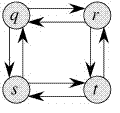
\includegraphics[width=0.2\linewidth]{images/LongestPath.png}

\subsection{Worked example: possible ways to sum coins}
Imagine there was a currency with coins of value 1, 5 and 7. The task is to list all possible combinations of these basic coins to obtain a total value of $n$.


Here is an idea how this could be implemented: 
Lets call our function \inlinecode{combs(n)}.
Add 1 to each list in the results of \inlinecode{combs(n-1)},
add 5 to each list in the results of \inlinecode{combs(n-5)}, 
and add 7 to each list in the results of \inlinecode{combs(n-7)}.


\begin{lstlisting}[language=python]

def combs(n):
	if n < 1:
		return []
	if n == 1:
		return [[1]]
	if n == 5:
		return [[1,1,1,1,1],[5]]
	if n == 7:
		return [[1,1,1,1,1,1,1],[5,1,1],[1,5,1],[1,1,5],[7]]

	list1 = combs(n-1)
	list5 = combs(n-5)
	list7 = combs(n-7)

	fullList = []
	for c in list1:
		fullList.append(c + [1])
	for c in list5:
		fullList.append(c + [5])
	for c in list7: 
		fullList.append(c + [7])

	return fullList

\end{lstlisting}

Now just add some caching, and you have an efficient algorithm as well. 

Verify that this idea shows overlapping subproblems
and that it shows optimal substructure

Proof that algorithm delivers correct results


counterexample: minimal number of coins


\subsection{A strategy for finding the recursion}

Dynamic programming tries to solve problems by breaking them apart into subproblems. But how do we find those subproblems?

The solution $S$ we are looking for should be obtained by some function $sol$.
$$ S = sol(para) $$

Try to find a way to split $S$ into a large part $S'$ and a small part $s$ \marginnote{In more advanced problems we might instead want to partition $S$ into several new sets $S'$ and $S''$}.
$$ S = S' + \{ s \} $$

The large part itself must be the result of $sol$ for some other set of parameters $para'$.
$$ S' = sol(para') $$





\subsection{Markow chains}

\subsection{Markov decision process with known state-transition-function}

MDPs are an extension of Markov chains, they add actions (allowing choice) and rewards (giving motivation). Conversely, if only one action exists for each state (e.g. "wait") and all rewards are the same (e.g. "zero"), a Markov decision process reduces to a Markov chain. 

An MDP is a tuple $(S, A, P_a, R_a)$, where 
\begin{itemize}
	\item $S$: finite set of states
	\item $A$: finite set of actions
	\item $P_a(s, s') = P(s_{t+1} = s' | s_t = s, a_t = a)$
	\item $R_a(s, s')$ is the immediate reward received after transitioning from $s$ to $s'$ through action $a$.
\end{itemize}

The goal is to find a policy $\pi(s) = a$ that maximizes the cumulative reward $\sum_{t=0}^\infty \gamma_t R_{a_t}(s_t, s_{t+1})$, where $\gamma_t$ is the discount-factor. The discount factor is used so that the decision maker favours taking actions early and doesn't postpone them indefinitely. 

Because of the Markov property, the optimal policy for this particular problem can indeed be written as a function of $s$ only, as assumed above.



\subsection{Reinforcement learning: MDP without explicitly known state-transition-function}

